\subsection{Theory}
%%%%%%%%%%%%%%%%%%%%%%%%%%%%%%%%%%%%%%%%%%%%%%%%%%%%%%%%%%%%%%%%%%%%%
\begin{frame}{Information flow dynamics: Structure of $\bar{W}_c$}
\begin{figure}
	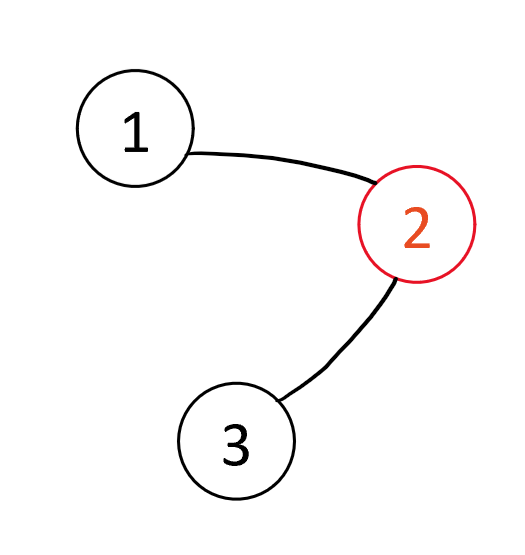
\includegraphics[width=0.3\textwidth]{figures/info_dyn_example.png}
	%\caption{Oil Spills}
	%\label{fig:oilspills}
\end{figure}
\begin{equation*}
\begin{split}
p_{k+1}&=\bar{W}_cp_k\\
&=\begin{bmatrix}
w_{11} & w_{12}&0\\
w_{21} & w_{22}&w_{22}\\
0 & w_{32}&w_{33}\\
\end{bmatrix}p_k
\end{split}
\end{equation*}
\begin{itemize}
\item Lot of work on designing weights for consensus e.g Metropolis-Hastings, equal-neighbor etc
\item We assume $w_{ij}\geq 0$ (Might be restrictive)
\end{itemize}
\end{frame}
%%%%%%%%%%%%%%%%%%%%%%%%%%%%%%%%%%%%%%%%%%%%%%%%%%%%%%%%%%%%%%%%%%%%%
\begin{frame}{Analysis of large scale positive systems}
	\textbf{\footnote{Rantzer, 2018}Theorem 1:}
	Consider a discrete-time autonomous system governed by 
	\begin{equation*}
	\begin{split}
	p_{k+1}=\bar{W}_cp_k, \\
	\end{split}
	\end{equation*}
	where $\bar{W}_c\geq 0$.		
	
	The following statements are equivalent
	\begin{itemize}
		\setlength\itemsep{0.3em}
		\item[(1)] $\bar{W}_c$ is Schur
		\item[(2)] $\lim\limits_{k\rightarrow \infty} p_k=\mathbf{0} \hspace{0.2cm} \forall p_0 \in \mathbb{R}^{n_p}$
		\item[(3)] $\exists \textnormal{ diagonal }P \succ 0 :\ P- \bar{W}_c^TP\bar{W}_c \succ 0$
		\item[(4)] $\exists \textnormal{ diagonal } P:\ \begin{bmatrix}
		P & \bar{W}_c^TP \\
		P\bar{W}_c& P
		\end{bmatrix} \succ 0$
	\end{itemize}	
\end{frame}
%%%%%%%%%%%%%%%%%%%%%%%%%%%%%%%%%%%%%%%%%%%%%%%%%%%%%%%%%%%%%%%%%%%%%
\begin{frame}{Scalable analysis}
\begin{itemize}	
	\item Diagonal P preserves the sparsity pattern in $\begin{bmatrix}
	P & \bar{W}_c^TP \\
	P\bar{W}_c& P
	\end{bmatrix}$
	\item Decompose the feasibility problem into small problems 
	\\(Uses the theory of chordal graphs and chordal graph extensions)\footnote{Papachristodoulou et al., 2012}
\end{itemize}
\end{frame}
%%%%%%%%%%%%%%%%%%%%%%%%%%%%%%%%%%%%%%%%%%%%%%%%%%%%%%%%%%%%%%%%%%%%%
\begin{frame}{Local analysis of agent dynamics}
\textcolor{blue}{Dynamics of agent $i$:}
\begin{equation*}
\begin{split}	
\begin{array}{ll}
x^i_{k+1}&=\bar{A}x^i_k+\bar{B}_pp^i_{k+1} + \bar{B}_ww^i_k \\
y^i_k &=\bar{C}x^i_k 
\end{array}
\end{split}
\end{equation*}
\pause
\textcolor{blue}{Generalized plant for agent $i$:}
\begin{figure}
	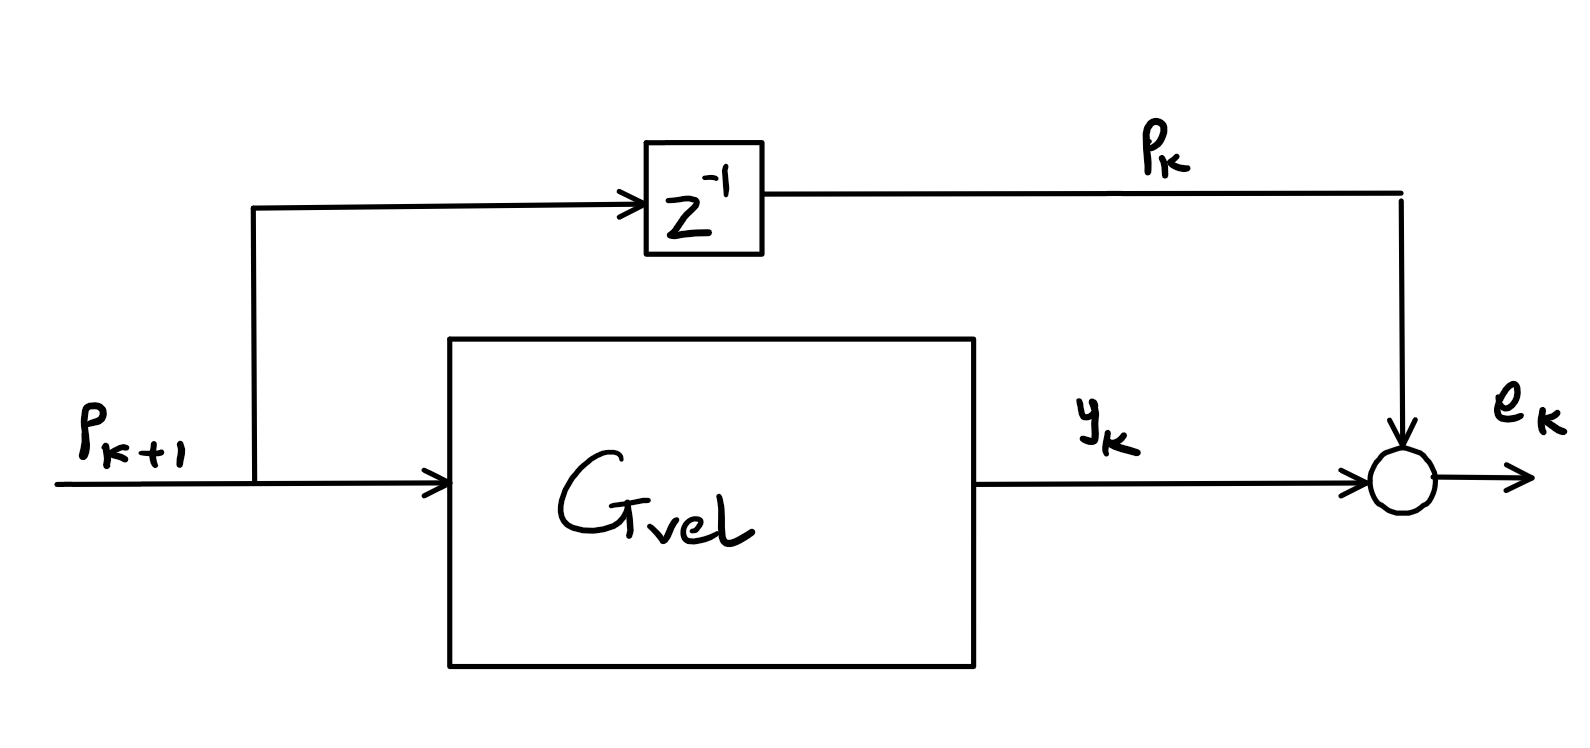
\includegraphics[width=0.45\textwidth]{figures/gen_plant_tf.png}
	%\caption{Oil Spills}
	%\label{fig:oilspills}
\end{figure}
\begin{equation*}\label{complete_closed_loop_aug_system}
\begin{split}
\begin{bmatrix}
z^i_{k+1}\\
\bar{z}^i_{k+1}
\end{bmatrix}
&=
\begin{bmatrix}
\bar{A} & 0\\
0 & 0\\
\end{bmatrix}
\begin{bmatrix}
z^i_k\\
\bar{z}^i_k
\end{bmatrix}
+
\begin{bmatrix}
\bar{B}_p\\
I 
\end{bmatrix}
p^i_{k+1}
+
\begin{bmatrix}
\bar{B}_w\\
0
\end{bmatrix}
w^i_k\\
\\
e^i_k &=
\begin{bmatrix}
-\bar{C} & I
\end{bmatrix}
\begin{bmatrix}
z^i_k\\
\bar{z}^i_k
\end{bmatrix}
\end{split}
\end{equation*}
\end{frame}
%%%%%%%%%%%%%%%%%%%%%%%%%%%%%%%%%%%%%%%%%%%%%%%%%%%%%%%%%%%%%%%%%%%%%
\begin{frame}{Local $l_2$ to $l_{\infty}$ control}
\textcolor{blue}{Generalized plant:}
\begin{equation}\label{eqn_open_loop_system}
\begin{split}
\eta_{k+1}&=\mathcal{A}\eta_k+\mathcal{B}_pp_k+\mathcal{B}_ww_k, \hspace{0.2cm}\eta_0=0\\
e_k &=\mathcal{C}\eta_k 
\end{split}
\end{equation}	
\pause
\textbf{Theorem 2:}
	For a discrete-time dynamical system governed by \eqref{eqn_open_loop_system}, 
	if $\exists K\succ0$, $\gamma_p \geq0$, $\gamma_w\geq0$ such that 
	\begin{equation} \label{eqn_LMI_Dissipativity1}
	\begin{split}	
	\hspace{1cm}
	\begin{bmatrix}
	\mathcal{A}^T\\
	\mathcal{B}_p^T\\
	\mathcal{B}_w^T\\
	\end{bmatrix}
	K
	\begin{bmatrix}
	\mathcal{A} & \mathcal{B}_p & \mathcal{B}_w
	\end{bmatrix}
	&\prec
	\begin{bmatrix}
	K & 0 & 0\\
	0 & \gamma_p^2 I&0\\
	0 & 0 &\gamma_w^2 I\\
	\end{bmatrix}\\
	\end{split}
	\end{equation}
	and
	\begin{equation}\label{eqn_LMI_output_bound1}
	\begin{bmatrix}
	K & \mathcal{C}^T \\
	* & I \\
	\end{bmatrix}\succ0, 
	\end{equation}
	then
	\begin{equation*}
	||e_k||_2^2\leq  \gamma_p^2||p||_{l_2}^2+\gamma_w^2||w||_{l_2}^2  \hspace{0.4cm} \forall w,p \in l_2,\ \forall k.
	\end{equation*}
\end{frame}
%%%%%%%%%%%%%%%%%%%%%%%%%%%%%%%%%%%%%%%%%%%%%%%%%%%%%%%%%%%%%%%%%%%%%
\begin{frame}{Local $l_2$ to $l_{\infty}$ control for agents}
\textbf{Proof:}	
	Condition (\ref{eqn_LMI_Dissipativity1}) is equivalent to the existence of $\epsilon>0$ such that $\forall \eta_k \in \mathbb{R}^{n_\eta},\forall w_k \in \mathbb{R}^{n_w}$, $\forall p_k \in \mathbb{R}^{n_p}$,
	\begin{equation*}
	\eta_{k+1}^TK\eta_{k+1}\leq\eta_{k}^TK\eta_{k}+(\gamma_p^2-\epsilon) ||p_{k}||_2^2+(\gamma_w^2-\epsilon) ||w_{k}||_2^2.
	\end{equation*}
	\pause
	Defining the storage function  $V_k=\eta_k^TK\eta_k$, we have  $\forall w_k \in \mathbb{R}^{n_w}$ and $\forall p_k \in \mathbb{R}^{n_p}$, 
	\begin{equation*}
	\begin{split}
	V_{k+1}&\leq V_{k}+\gamma_p^2 ||p_{k}||_2^2+\gamma_w^2 ||w_{k}||_2^2\\
	\pause
	&\leq V_{0}+\gamma_p^2 \sum_{i=0}^{k}||p_{i}||_2^2+\gamma_w^2 \sum_{i=0}^{k}||w_{i}||_2^2
	\end{split}	
	\end{equation*}
	\pause
	With zero initial conditions, and $\forall w,p \in l_2$, 
	\begin{equation} \label{eqn_dissipativity}
	V_{k}\leq\gamma_p^2\sum_{i=0}^{k-1}||p_i||_2^2+\gamma_w^2\sum_{i=0}^{k-1}||w_i||_2^2\leq\gamma_p^2||p||_{l_2}^2+\gamma_w^2||w||_{l_2}^2. 
	\end{equation}
\end{frame}
%%%%%%%%%%%%%%%%%%%%%%%%%%%%%%%%%%%%%%%%%%%%%%%%%%%%%%%%%%%%%%%%%%%%%
\begin{frame}{Local $l_2$ to $l_{\infty}$ control for agents}
\textbf{Proof(ctd):} Condition (\ref{eqn_LMI_output_bound1}) can be converted using the Schur complement to
\begin{equation}
K-C^TC\succ0
\end{equation}
which is equivalent to 
\begin{equation*}
V_k=\eta_k^TK\eta_k\geq\eta_k^TC^TC\eta_k=e_k^Te_k \hspace{0.3cm}\forall \eta_k \in \mathbb{R}^{n_\eta}
\end{equation*}
which together with equation (\ref{eqn_dissipativity}) implies 
\begin{equation*}
||e_k||_2^2\leq V_k \leq \gamma_p^2||p||_{l_2}^2+\gamma_w^2||w||_{l_2}^2.  
\end{equation*}
$\forall w,p \in l_2$, $\forall k$
\end{frame}
%%%%%%%%%%%%%%%%%%%%%%%%%%%%%%%%%%%%%%%%%%%%%%%%%%%%%%%%%%%%%%%%%%%%%
\begin{frame}{Complete interconnected system: Analysis}
\begin{equation}\label{eqn:full_system_closed_loop}
\begin{split}
&\hspace{0.78cm}p_{k+1}=\bar{W}_cp_k \\
\forall i:
~~&\left\{
\begin{array}{ll}
x^i_{k+1}&=\bar{A}x^i_k+\bar{B}_pp^i_{k+1} + \bar{B}_ww^i_k \\
y^i_k &=\bar{C}x^i_k 
\end{array}
\right.
\end{split}
\end{equation}
For the interconnected system (\ref{eqn:full_system_closed_loop}), consider the following three LMIs:
\begin{equation} \label{eqn_LMI_pos_analysis}
%\exists \textnormal{ diagonal } P :
\left[
\begin{array}{c|c}
\alpha^2 P & \bar{W}_c^TP \\
\hline \\
P\bar{W}_c& P
\end{array}\right] \succ 0,
\end{equation} 
\begin{equation} \label{eqn_LMI_Dissipativity}
\begin{split}	
\hspace{1cm}
\begin{bmatrix}
\mathcal{A}^T\\
\mathcal{B}_p^T\\
\mathcal{B}_w^T\\
\end{bmatrix}
K
\begin{bmatrix}
\mathcal{A} & \mathcal{B}_p & \mathcal{B}_w
\end{bmatrix}
&\prec
\begin{bmatrix}
K & 0 & 0\\
0 & \gamma_p^2 I&0\\
0 & 0 &\gamma_w^2 I\\
\end{bmatrix}\\
\end{split}
\end{equation}
\begin{equation}\label{eqn_LMI_output_bound}
\begin{bmatrix}
K & \mathcal{C}^T \\
* & I \\
\end{bmatrix}\succ0, 
\end{equation}
\end{frame}
%%%%%%%%%%%%%%%%%%%%%%%%%%%%%%%%%%%%%%%%%%%%%%%%%%%%%%%%%%%%%%%%%%%%%
\begin{frame}{Complete interconnected system: Analysis}
\textbf{Theorem 3:} If for $0\leq \alpha< 1$, $\exists P$ diagonal and $\exists K \succ 0$ and $\gamma_p\geq0$, $\gamma_w\geq0$ such that the LMIs \eqref{eqn_LMI_pos_analysis}, \eqref{eqn_LMI_Dissipativity} and \eqref{eqn_LMI_output_bound} are satisfied,
then the interconnected system is stable such that for all bounded disturbances $||w^i||_{l_2}\leq \beta$,
\begin{equation}\label{eqn:stability guarantee}
||y_k^i||_2\leq (\alpha^k+\frac{\gamma_p}{1-\alpha})\sqrt{\textnormal{cond}(P)}||p_0||_2+\gamma_w\beta
\end{equation} $\forall k$.

Moreover
\begin{equation}\label{perf_bound1}
\begin{split}
\nu_k\leq\mu_k+\frac{\gamma_p}{1-\alpha}\sqrt{\frac{\textnormal{cond}(P)}{N}}||p_0||_2+\gamma_w\beta.
\end{split}
\end{equation}	
and 
\begin{equation}\label{perf_bound2}
J_k\leq M_k+\alpha^{2k}\frac{d_{\textnormal{max}}\gamma_p^2}{|\mathcal{E}|}\textnormal{cond}(P)||p_0||_2^2+\gamma_w^2 \beta^2.
\end{equation}
\end{frame}
%%%%%%%%%%%%%%%%%%%%%%%%%%%%%%%%%%%%%%%%%%%%%%%%%%%%%%%%%%%%%%%%%%%%%
\begin{frame}{Complete interconnected system: Analysis}
\textbf{Key arguments in the proof}
\begin{itemize}
\item Application of Theorem 1 and Theorem 2
\item Convergence result of geometric series
\item Other estimates on norms such as $\frac{1}{\sqrt{N}}||p||_1\leq||p_k||_2\leq||p_k||_1$
\end{itemize}
\end{frame}
%%%%%%%%%%%%%%%%%%%%%%%%%%%%%%%%%%%%%%%%%%%%%%%%%%%%%%%%%%%%%%%%%%%%%
\begin{frame}{Analysis to Synthesis}

Conisder the control variable matrices $F_1$, $F_2$ and a diagonal matrix $E$ of appropriate sizes forming the closed loop matrices
\begin{itemize}
\item $\bar{W}_c=I-EL_c$ where $L_c$ is the perturbed Laplacian matrix
\item $\bar{A}=A+B_uF_1$
\item $\bar{B}_p=B_uF_2$
\end{itemize}	
\end{frame}
%%%%%%%%%%%%%%%%%%%%%%%%%%%%%%%%%%%%%%%%%%%%%%%%%%%%%%%%%%%%%%%%%%%%%
\begin{frame}{Analysis to Synthesis}
	Now consider the set of LMIs:
	\begin{equation}\label{eqn:LMI_synthesis_cond_1}
	\left[
	\begin{array}{c|c|c}
	\begin{array}{ccc}
	R & 0\\
	0 & S 
	\end{array} & * & * \\
	\hline
	0 & \begin{array}{ccc}
	\gamma_p^2I & 0\\
	0 & \gamma_w^2I\\
	\end{array} & *\\
	\hline
	\begin{array}{ccc}
	AR+B_uY & 0\\
	0 & 0 
	\end{array} & 
	\begin{array}{ccc}
	B_uF_2 & B_w\\
	I & 0 
	\end{array} & 
	\begin{array}{ccc}
	R & 0\\
	0 & S 
	\end{array}\\
	\end{array}
	\right]\succ0,
	\end{equation}
	\begin{equation}\label{eqn:LMI_synthesis_cond_2}
	\left[
	\begin{array}{c|c}
	\begin{array}{ccc}
	R & 0\\
	0 & S 
	\end{array} & *\\
	\hline
	\begin{array}{ccc}
	-CR & S
	\end{array} & I \\
	\end{array}\right]\succ 0,
	\end{equation}
	and 
	\begin{equation} \label{eqn:LMI_pos_synthesis}
	\begin{bmatrix}
	\alpha^2 P & P^T-L_c^TX^T \\
	P-XL_c& P
	\end{bmatrix} \succ 0,
	\end{equation}
\end{frame}
%%%%%%%%%%%%%%%%%%%%%%%%%%%%%%%%%%%%%%%%%%%%%%%%%%%%%%%%%%%%%%%%%%%%%
\begin{frame}{Analysis to Synthesis}
\textbf{Theorem 4:}
	If $\exists R\succ0$, $S\succ0$, $Y$, $F_2$ and $\gamma >0$, and diagonal matrices $P$ and $X$ such that for an $0\leq\alpha<1$, the LMIs \eqref{eqn:LMI_synthesis_cond_1}, \eqref{eqn:LMI_synthesis_cond_2} and \eqref{eqn:LMI_pos_synthesis} hold,
	
	then $F_1=YR^{-1}$, $F_2$ and $E=P^{-1}X$ stabilize the networked system in the sense of (\ref{eqn:stability guarantee}) and the performance bounds (\ref{perf_bound1}) and (\ref{perf_bound2}) hold.
\pause

\textbf{Key arguments in the proof}
\begin{itemize}
	\item Imposition of a structure on the Lyapunov matrix $K=\begin{bmatrix}R&0\\0&S
	\end{bmatrix}$
	\item Introduction of new variables $Y=F_1R$ and $X=PE$
	\item A similarity transformation and Schur complement for linearization 
\end{itemize}
\end{frame}
%%%%%%%%%%%%%%%%%%%%%%%%%%%%%%%%%%%%%%%%%%%%%%%%%%%%%%%%%%%%%%%%%%%%%
\begin{frame}{An extreme case for insight}
\textbf{Agent dynamics:} $i \in \{1,2,\cdots N\}$
\begin{equation}
\begin{split}
x^i_{k+1}&=ax^i_k+b_uu^i_k+b_ww^i_k \\
y^i_k&=x^i_k
\end{split}
\end{equation}
\pause
\textbf{Controller structure:}
\begin{equation}
u^i_k=f_1x^i_k+f_2p^i_{k+1}.
\end{equation}
\pause
With $f_1={-a}/{b_u}$ and $f_2={1}/{b_u}$, closed loop agent dynamics are
\begin{equation}
\begin{split}
x^i_{k+1}&=p^i_{k+1}+b_ww^i_k \\
y^i_k&=x^i_k
\end{split}
\end{equation}
\pause
min $\gamma_p$ subject to constraints (\ref{eqn_LMI_Dissipativity}) gives $\gamma_p^*=0$. 
%$$\textnormal{inf}~ \gamma_p ~~\textnormal{s.t}~~$$
%This can be easily seen intuitively by observing that we have perfect tracking for arbitrary $p_k$ whenever $w_k\equiv0$.

\pause
\begin{align}
\label{eqn:stability guarantee_sp_case_1}
||y_k^i||_2&\leq \alpha^k\sqrt{\textnormal{cond}(P)}||y_0||_2+\gamma_w\beta\\
\label{perf_bound1_sp_case1}
\nu_k&\leq\mu_k+\gamma_w \beta \\
\label{perf_bound2_sp_case1}
J_k&\leq M_k+\gamma_w^2 \beta^2.
\end{align}
\end{frame}
